% !TEX program = xelatex
% AY2015 材料力学 解答例（同志社 生命医科学 医工学コース 院試）
% 問題・図は 01_exams/2015/tex を土台に、参考/ の粒度で解答を付した。
\documentclass[11pt,a4paper]{article}
\usepackage{../../00_common/preamble}
\usetikzlibrary{positioning,arrows.meta,calc,patterns,decorations.pathmorphing}

\title{材料力学 AY2015 解答例}
\author{}
\date{}

\begin{document}
\maketitle

\noindent\textbf{符号規約}：反力・たわみは上向きを正，集中荷重 $P$・分布荷重 $f_0$ は下向き．
せん断力 $Q$ は断面左側に働く上向き外力の和，曲げモーメント $M$ は下に凸（さがり）を正とし，
たわみの基礎式は $EI\,\dfrac{d^2v}{dx^2}=M(x)$ を用いる．応力は引張りを正，トルクは右ねじを正とする．

%====================================================================
\section*{〔I〕}

図1に示す片持ちはりの自由端 A に, はりの軸線に垂直方向に固定された剛体棒（水平方向，長さ $L/2$）の
先端に, 鉛直方向下向きに外力 $P$ が加わる場合について答えよ. はりの縦弾性係数を $E$, 横弾性係数を $G$,
断面形状を直径 $d$ の円形とする.

\begin{center}
\begin{tikzpicture}[>=Latex]
  \draw (1.0,0.4) -- (7.0,0.4);
  \draw (1.0,-0.4) -- (7.0,-0.4);
  \draw (1.0,0) ellipse (0.22 and 0.4);
  \fill[pattern=north east lines] (7.0,-1.3) -- (7.0,1.3) -- (8.0,1.7) -- (8.0,-0.9) -- cycle;
  \draw (7.0,-1.3) -- (7.0,1.3) -- (8.0,1.7) -- (8.0,-0.9) -- cycle;
  \draw[->] (1.0,0) -- (2.2,0) node[above]{$x$};
  \draw[->] (1.0,0) -- (1.0,1.3) node[left]{$y$};
  \draw[->] (1.0,0) -- (0.35,0.55) node[above left]{$z$};
  \node[below left] at (1.0,-0.2) {A};
  \node at (6.7,0.75) {B};
  \draw[line width=1.4pt] (1.0,-0.1) -- (1.55,-1.5);
  \node[fill=white,inner sep=1pt] at (0.78,-1.0) {$L/2$};
  \draw[->,very thick] (1.55,-1.5) -- (1.55,-2.6) node[below]{$P$};
  \draw[<->] (1.0,1.55) -- (7.0,1.55) node[midway,fill=white]{$L$};
  \begin{scope}[shift={(-1.3,-0.2)}]
    \draw (0,0) circle (0.5);
    \draw[->] (0,-0.5) -- (0,0.9) node[left]{$y$};
    \draw[->] (0,0) -- (-1.0,0) node[above]{$z$};
    \draw[<->] (-0.5,-0.75) -- (0.5,-0.75) node[midway,fill=white,font=\scriptsize]{$d$};
  \end{scope}
  \begin{scope}[shift={(7.3,-2.4)}]
    \draw (0,0) circle (0.5);
    \draw[dash dot] (-0.8,0) -- (0.8,0);
    \draw[dash dot] (0,-0.8) -- (0,0.8);
    \fill (0,-0.5) circle (1.6pt);
    \node[right] at (-0.9,0.5) {C};
    \draw[->] (-0.75,0.45) -- (-0.05,-0.45);
    \node at (0,-1.1) {B 断面};
  \end{scope}
\end{tikzpicture}

\vspace{1mm}
図1
\end{center}

\subsection*{解答}

\noindent\textbf{(1)}\quad 荷重 $P$ ははり軸線（$x$ 軸）から水平に $L/2$ 離れた点に下向きに作用する．
これを自由端 A の軸線上へ移すと，\textbf{下向きの力 $P$} と，剛体棒のうでによる
\textbf{軸まわりのトルク $T=P\cdot\dfrac{L}{2}$} に等価となる．
固定端 B でこれらをすべて支える．鉛直力のつり合い，B まわりの曲げモーメントのつり合い，
および軸まわりのトルクのつり合いより
\[
  R_B = P,\qquad M_B = P\cdot L,\qquad T_B = P\cdot \frac{L}{2}.
\]
\[
  \ans{\,R_B = P\ (\text{上向き}),\quad M_B = PL\ (\text{曲げ反モーメント}),\quad T_B = \dfrac{PL}{2}\ (\text{反トルク})\,}
\]
検算：自由端 A の力 $P$ が固定端まで距離 $L$ を隔てるから曲げ反モーメントは $P L$，
うで $L/2$ のトルクは $P L/2$ で，外力系と過不足なくつり合う ✓．

\medskip
\noindent\textbf{(2)}\quad 座標 $x$ を自由端 A から固定端 B へ向けてとる（$0\le x\le L$）．
はりにはせん断を伴う曲げと一定トルクが同時に作用する．断面左側のつり合いより
\[
  Q(x) = P\ (\text{一定}),\qquad M(x) = P\,x,\qquad T(x) = \frac{PL}{2}\ (\text{一定}).
\]
端点の値は $M(0)=0$（自由端），$M(L)=PL$（固定端）である．
\[
  \ans{\,Q(x)=P,\qquad M(x)=Px\ \ (0\le x\le L),\qquad T(x)=\dfrac{PL}{2}\,}
\]

\begin{center}
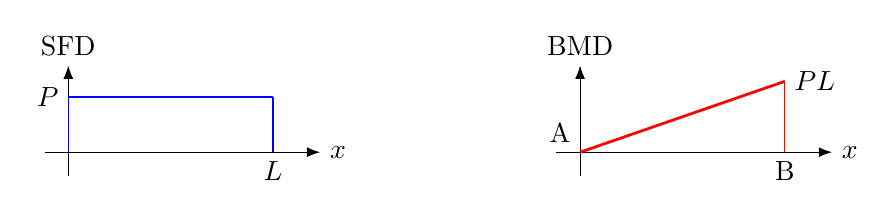
\begin{tikzpicture}[>=Latex,scale=1.0]
  \def\L{2.6}
  \begin{scope}
    \draw[->] (-0.3,0) -- (\L+0.6,0) node[right]{$x$};
    \draw[->] (0,-0.3) -- (0,1.1) node[above]{SFD};
    \draw[line width=1pt,blue] (0,0.7) -- (\L,0.7);
    \draw[blue] (0,0)--(0,0.7); \draw[blue] (\L,0)--(\L,0.7);
    \node[left] at (0,0.7) {$P$};
    \node[below] at (\L,0) {$L$};
  \end{scope}
  \begin{scope}[xshift=6.5cm]
    \draw[->] (-0.3,0) -- (\L+0.6,0) node[right]{$x$};
    \draw[->] (0,-0.3) -- (0,1.1) node[above]{BMD};
    \draw[line width=1pt,red] (0,0) -- (\L,0.9);
    \draw[red] (\L,0)--(\L,0.9);
    \node[right] at (\L,0.9) {$PL$};
    \node[above left] at (0,0) {A}; \node[below] at (\L,0) {B};
  \end{scope}
\end{tikzpicture}
\end{center}

\medskip
\noindent\textbf{(3)}\quad 固定端 B では $M_B=PL$，$T_B=PL/2$．円形断面（直径 $d$）の諸量は
\[
  I=\frac{\pi d^4}{64},\qquad I_p=J=\frac{\pi d^4}{32},\qquad c=\frac{d}{2}.
\]
点 C は断面の最下縁（曲げの中立軸 $z$ から最も離れた縁）にある．
曲げによる軸方向応力（大きさ）は
\[
  \sigma=\frac{M_B\,c}{I}=\frac{PL\cdot (d/2)}{\pi d^4/64}=\frac{32PL}{\pi d^3}.
\]
ねじりによるせん断応力は
\[
  \tau=\frac{T_B\,c}{J}=\frac{(PL/2)(d/2)}{\pi d^4/32}=\frac{8PL}{\pi d^3}.
\]
なお曲げに伴う横（断面内）せん断応力は中立軸で最大・最外縁で $0$ であるから，
最外縁の点 C ではねじりせん断のみが残る．
\[
  \ans{\,\sigma=\dfrac{32PL}{\pi d^3}\ (\text{軸方向，C は圧縮側}),\qquad \tau=\dfrac{8PL}{\pi d^3}\ (\text{ねじり})\,}
\]
検算：$\sigma/\tau = (32PL)/(8PL)=4$．これは $M_B/T_B=PL/(PL/2)=2$ に断面係数比
$Z/Z_p=(I/c)\big/(J/c)=I/J=1/2$ の逆数 $2$ を掛けた $2\times2=4$ と一致する ✓．

\medskip
\noindent\textbf{(4)}\quad 点 C の応力状態は，軸方向応力 $\sigma_x=\sigma$，円周方向応力 $\sigma_y=0$，
せん断応力 $\tau_{xy}=\tau$ の平面応力である（大きさで表す）．
モールの応力円の中心と半径は
\[
  \sigma_{\text{c}}=\frac{\sigma_x+\sigma_y}{2}=\frac{\sigma}{2}=\frac{16PL}{\pi d^3},\qquad
  R=\sqrt{\Big(\frac{\sigma}{2}\Big)^2+\tau^2}
   =\sqrt{16^2+8^2}\,\frac{PL}{\pi d^3}=\frac{8\sqrt{5}\,PL}{\pi d^3}.
\]
主応力と最大せん断応力は
\[
  \sigma_{1,2}=\sigma_{\text{c}}\pm R,\qquad \tau_{\max}=R.
\]
\[
  \ans{\;\sigma_1=\dfrac{(16+8\sqrt5)PL}{\pi d^3},\quad
        \sigma_2=\dfrac{(16-8\sqrt5)PL}{\pi d^3},\quad
        \tau_{\max}=\dfrac{8\sqrt5\,PL}{\pi d^3}\;}
\]

\begin{center}
\begin{tikzpicture}[>=Latex,scale=0.85]
  \def\u{0.2}      % 1単位 = PL/(pi d^3) を 0.2cm に
  \def\cx{16}      % 中心
  \def\R{17.889}   % 8 sqrt5
  \draw[->] (-2*\u,0) -- ({(\cx+\R+5)*\u},0) node[right]{$\sigma$};
  \draw[->] (0,{-(\R+4)*\u}) -- (0,{(\R+4)*\u}) node[above]{$\tau$};
  \draw[line width=1pt,blue] ({\cx*\u},0) circle ({\R*\u});
  \fill ({\cx*\u},0) circle (1.2pt);
  % 応力点 (sigma_x, +tau) と (0, -tau)
  \fill ({32*\u},{8*\u}) circle (1.2pt) node[right]{\scriptsize $(\sigma,\,\tau)$};
  \fill (0,{-8*\u}) circle (1.2pt) node[left]{\scriptsize $(0,\,-\tau)$};
  \draw[dashed] ({32*\u},{8*\u}) -- (0,{-8*\u});
  % 主応力点
  \fill ({(\cx+\R)*\u},0) circle (1.2pt) node[above right]{\scriptsize $\sigma_1$};
  \fill ({(\cx-\R)*\u},0) circle (1.2pt) node[above left]{\scriptsize $\sigma_2$};
  \node[below] at ({\cx*\u},0) {\scriptsize $\sigma/2$};
  \node[above] at ({\cx*\u},{\R*\u}) {\scriptsize $\tau_{\max}=R$};
\end{tikzpicture}

\vspace{1mm}
モールの応力円（単位 $PL/(\pi d^3)$）
\end{center}
検算：$\sigma_1+\sigma_2=2\sigma_{\text{c}}=\dfrac{32PL}{\pi d^3}=\sigma_x+\sigma_y$（不変量），
また $\sigma_1\sigma_2=(16^2-320)\big(\tfrac{PL}{\pi d^3}\big)^2=-64\big(\tfrac{PL}{\pi d^3}\big)^2=-\tau^2$
で $\sigma_x\sigma_y-\tau_{xy}^2$ に一致する ✓．

%====================================================================
\clearpage
\section*{〔II〕}

図2に示す突き出しはりの自由端 C に集中荷重 $P$, AB 間に等分布荷重 $f_0$ が負荷される場合について答えよ.
縦弾性係数を $E$, 断面形状を幅 $b$, 高さ $h$ の長方形とする. ただし $\,P<f_0L/4\,$ とする.
A 端は壁に固定（固定端），B はローラー支持である．

\begin{center}
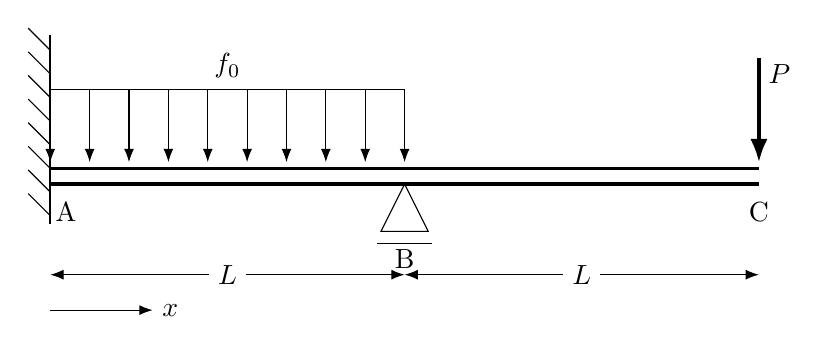
\begin{tikzpicture}[>=Latex]
  \draw[thick] (0,-0.6) -- (0,1.8);
  \foreach \y in {-0.5,-0.2,...,1.75} {\draw (0,\y) -- (-0.28,\y+0.28);}
  \draw[line width=1.2pt] (0,0.1) -- (9,0.1);
  \draw[line width=1.2pt] (0,-0.1) -- (9,-0.1);
  \draw (0,1.1) -- (4.5,1.1);
  \foreach \x in {0,0.5,...,4.5} {\draw[->] (\x,1.1) -- (\x,0.18);}
  \node at (2.25,1.4) {$f_0$};
  \draw (4.5,-0.1) -- (4.2,-0.7) -- (4.8,-0.7) -- cycle;
  \draw (4.15,-0.85) -- (4.85,-0.85);
  \draw[->,very thick] (9,1.5) -- (9,0.18);
  \node[right] at (9,1.3) {$P$};
  \node at (0.2,-0.45) {A};
  \node at (4.5,-1.05) {B};
  \node at (9,-0.45) {C};
  \draw[<->] (0,-1.25) -- (4.5,-1.25) node[midway,fill=white]{$L$};
  \draw[<->] (4.5,-1.25) -- (9,-1.25) node[midway,fill=white]{$L$};
  \draw[->] (0,-1.7) -- (1.3,-1.7) node[right]{$x$};
\end{tikzpicture}

\vspace{1mm}
図2
\end{center}

\subsection*{解答}

\noindent\textbf{(1)}\quad 座標 $x$ を A（$x=0$）から C（$x=2L$）へとる．B は $x=L$．
固定端 A に上向き反力 $R_A$ と反モーメント $M_A$（壁が与えるホギング向きを正），
ローラー B に上向き反力 $R_B$ を仮定する（ローラーゆえ反モーメントなし）．
未知数は $R_A,M_A,R_B$ の 3 個に対し，つり合い式は 2 本なので，この系は 1 次不静定である．
鉛直方向の力のつり合いと，A まわりのモーメントのつり合いは
\[
  R_A+R_B-f_0L-P=0,\qquad
  M_A + R_B\,L - f_0 L\cdot\frac{L}{2} - P\cdot 2L = 0.
\]
\[
  \ans{\;R_A+R_B = f_0L+P,\qquad M_A = f_0\frac{L^2}{2}+2PL - R_B L\;}
\]
不足する 1 式はたわみの境界条件（B でたわみ $0$）から (3) で与え，反力を確定する．

\medskip
\noindent\textbf{(2)}\quad 区間ごとに断面左側のつり合いをとる（反力は $R_A,M_A,R_B$ のまま残す）．

\noindent(I)\ $0\le x\le L$（区間 AB）：
\[
  Q(x)=R_A-f_0x,\qquad M(x)=-M_A+R_A x-\frac{f_0}{2}x^2 .
\]
(II)\ $L\le x\le 2L$（区間 BC）：この区間には分布荷重がなく，右側には自由端 C の $P$ のみが残るので
\[
  Q(x)=P,\qquad M(x)=-P\,(2L-x)=Px-2PL .
\]
反力を (3) の結果
\[
  R_A=\frac{5}{8}f_0L-\frac{3}{2}P,\qquad R_B=\frac{3}{8}f_0L+\frac{5}{2}P,\qquad M_A=\frac{f_0L^2}{8}-\frac{PL}{2}
\]
で表すと，区間 AB の曲げモーメントは
\[
  M(x)=-\frac{f_0}{2}x^2+\Big(\frac{5}{8}f_0L-\frac{3}{2}P\Big)x+\Big(\frac{PL}{2}-\frac{f_0L^2}{8}\Big).
\]
代表値は $M(0)=\dfrac{PL}{2}-\dfrac{f_0L^2}{8}\,(<0$, ホギング$)$，$M(L)=-PL$，$M(2L)=0$ である．
\[
  \ans{\;Q(x)=\begin{cases}\dfrac{5}{8}f_0L-\dfrac{3}{2}P-f_0x & (0\le x\le L)\\[2mm] P & (L\le x\le 2L)\end{cases}\;}
\]
\[
  \ans{\;M(x)=\begin{cases}-\dfrac{f_0}{2}x^2+\big(\tfrac58 f_0L-\tfrac32P\big)x+\big(\tfrac{PL}{2}-\tfrac{f_0L^2}{8}\big) & (0\le x\le L)\\[2mm] Px-2PL & (L\le x\le 2L)\end{cases}\;}
\]

\begin{center}
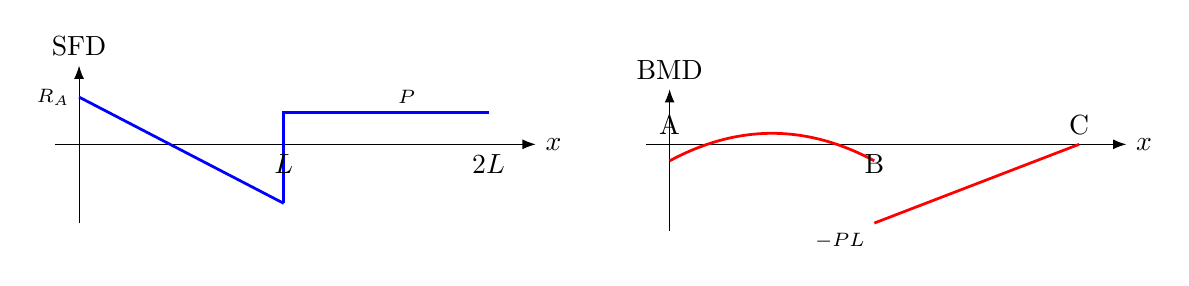
\begin{tikzpicture}[>=Latex,scale=1.0]
  \def\L{2.6}
  \begin{scope}
    \draw[->] (-0.3,0) -- (2*\L+0.6,0) node[right]{$x$};
    \draw[->] (0,-1.0) -- (0,1.0) node[above]{SFD};
    % 区間AB: x=0 で R_A>0, 直線で下降, x=L で R_A-f0L = -3f0L/8-3P/2 <0
    \draw[line width=1pt,blue] (0,0.6) -- (\L,-0.75);
    % B でローラー反力により上昇, 区間BC で一定 = P >0
    \draw[line width=1pt,blue] (\L,-0.75) -- (\L,0.4) -- (2*\L,0.4);
    \node[left] at (0,0.6) {\scriptsize $R_A$};
    \node[above] at (1.6*\L,0.4) {\scriptsize $P$};
    \node[below] at (\L,0) {$L$}; \node[below] at (2*\L,0) {$2L$};
  \end{scope}
  \begin{scope}[xshift=7.5cm]
    \draw[->] (-0.3,0) -- (2*\L+0.6,0) node[right]{$x$};
    \draw[->] (0,-1.1) -- (0,0.7) node[above]{BMD};
    % 区間AB: x=0 で M0<0(小さい負), 内部で正の極大, x=L で -PL(負,谷)
    \draw[line width=1pt,red,smooth,samples=40,domain=0:1]
      plot ({\L*\x},{0.35*(-(\x*\x)*4 + 4.0*\x -0.6)});
    % 区間BC: -PL から 0 へ直線
    \draw[line width=1pt,red] (\L,-1.0) -- (2*\L,0);
    \node[below left] at (\L,-1.0) {\scriptsize $-PL$};
    \node[above] at (0,0) {A}; \node[below] at (\L,0) {B}; \node[above] at (2*\L,0) {C};
  \end{scope}
\end{tikzpicture}
\end{center}
（BMD：区間 AB は上に凸の放物線で，A 端は小さな負，途中で正の極大を経て B で $-PL$ の谷．区間 BC は $-PL$ から $0$ への直線．）

\medskip
\noindent\textbf{(3)}\quad たわみの基礎式 $EI\,v''=M(x)$ を各区間で2回積分する．
区間 AB（$0\le x\le L$）では，
\[
  EI\,v_1' = -\frac{f_0}{6}x^3+\Big(\frac{5}{16}f_0L-\frac34P\Big)x^2+\Big(\frac{PL}{2}-\frac{f_0L^2}{8}\Big)x+C_1,
\]
\[
  EI\,v_1 = -\frac{f_0}{24}x^4+\Big(\frac{5}{48}f_0L-\frac14P\Big)x^3+\frac12\Big(\frac{PL}{2}-\frac{f_0L^2}{8}\Big)x^2+C_1x+C_2 .
\]
固定端の境界条件 $v_1(0)=0,\ v_1'(0)=0$ より $C_1=C_2=0$．
区間 BC（$L\le x\le 2L$）では $M=Px-2PL$ より
\[
  EI\,v_2' = \frac{P}{2}x^2-2PL\,x+C_3,\qquad
  EI\,v_2 = \frac{P}{6}x^3-PL\,x^2+C_3x+C_4 .
\]
接続条件 $v_1'(L)=v_2'(L)$ と，ローラー支持 $v_1(L)=0,\ v_2(L)=0$ の3条件から，未知の冗長反力を含めて確定すると
\[
  R_B=\frac{3}{8}f_0L+\frac52P,\quad
  C_3=\frac{f_0L^3}{48}+\frac{5PL^2}{4},\quad
  C_4=-\frac{f_0L^4}{48}-\frac{5PL^3}{12},
\]
であり，これより (2) に示した
$R_A=\tfrac58 f_0L-\tfrac32P,\ M_A=\tfrac{f_0L^2}{8}-\tfrac{PL}{2}$ が得られる．
\[
  \ans{\;R_A=\frac{5}{8}f_0L-\frac{3}{2}P,\quad R_B=\frac{3}{8}f_0L+\frac{5}{2}P,\quad M_A=\frac{f_0L^2}{8}-\frac{PL}{2}\ (\text{ホギング})\;}
\]
たわみ角・たわみ曲線は
\[
  \ans{\;EI\,v_1=-\frac{f_0}{24}x^4+\Big(\frac{5}{48}f_0L-\frac14P\Big)x^3+\frac12\Big(\frac{PL}{2}-\frac{f_0L^2}{8}\Big)x^2\;}
\]
\[
  \ans{\;EI\,v_2=\frac{P}{6}x^3-PL\,x^2+\Big(\frac{f_0L^3}{48}+\frac{5PL^2}{4}\Big)x-\frac{f_0L^4}{48}-\frac{5PL^3}{12}\;}
\]
自由端 C（$x=2L$）のたわみは
\[
  EI\,v_2(2L)=\frac{P}{6}(2L)^3-PL(2L)^2+\Big(\frac{f_0L^3}{48}+\frac{5PL^2}{4}\Big)2L-\frac{f_0L^4}{48}-\frac{5PL^3}{12}
  =\frac{f_0L^4}{48}-\frac{7PL^3}{12}.
\]
\[
  \ans{\;v_C=\frac{1}{EI}\left(\frac{f_0L^4}{48}-\frac{7PL^3}{12}\right),\qquad I=\frac{bh^3}{12}\;}
\]
検算：$P=0$（C の荷重なし）とすると $R_B=\dfrac38 f_0L$，$M_A=\dfrac{f_0L^2}{8}$ となり，
等分布荷重を受ける一端固定・他端ローラー支持はり（プロップド片持ちはり）の既知解に一致する ✓．
また両支点条件 $v_1(0)=0,\ v_1'(0)=0,\ v_1(L)=0,\ v_2(L)=0$ と接続 $v_1'(L)=v_2'(L)$ がすべて満たされる ✓．

%====================================================================
\clearpage
\section*{〔III〕}

図3に示す組合せ棒について答えよ. 丸棒 1（直径 $d$, 縦弾性係数 $E$）は上部 A--B（長さ $L/2$），
丸棒 2（直径 $2d$, 縦弾性係数 $3E$）は下部 B--C（長さ $L/2$）にあり，両者は B で接合される．
円管 3（内径 $4d$, 外径 $6d$, 縦弾性係数 $2E$）は全長 $L$ にわたる．組合せ棒の下面は固定され，
上面も剛体円板で固定される（両端固定）．2 本の丸棒の接合点 B に下向きの外力 $P$ が作用し，
剛体板は平行を保つ．横弾性係数はすべて $G$ とする．

\begin{center}
% 断面図（同心円）
\begin{tikzpicture}[>=Latex,scale=0.9]
  \begin{scope}
    \clip (0,0) circle (1.8); \fill[pattern=north east lines] (-2,-2) rectangle (2,2);
    \fill[white] (0,0) circle (1.2);
  \end{scope}
  \draw (0,0) circle (1.8); \draw (0,0) circle (1.2);
  \fill[gray!45] (0,0) circle (0.6); \draw (0,0) circle (0.6);
  \fill[white] (0,0) circle (0.3); \draw (0,0) circle (0.3);
  \node at (0,0.95) {\footnotesize 丸棒 1};
  \draw[->] (0,0.82) -- (0,0.16);
  \node at (1.75,-1.55) {\footnotesize 丸棒 2};
  \draw[->] (1.3,-1.3) -- (0.4,-0.42);
  \node[below left] at (-1.45,-1.2) {\footnotesize 円管 3};
  \draw[->] (-1.25,-1.05) -- (-0.95,-0.85);
  \draw[->,line width=1pt] (1.4,1.6) arc (55:-35:2.1) node[midway,right]{$T$};
\end{tikzpicture}
\hspace{8mm}
% 縦断面図
\begin{tikzpicture}[>=Latex,scale=0.9]
  \draw[thick] (-2.0,0) -- (2.0,0);
  \foreach \x in {-1.9,-1.6,...,1.95} {\draw (\x,0) -- (\x-0.25,-0.25);}
  \draw[line width=2pt] (-2.0,5.0) -- (2.0,5.0);
  \foreach \x in {-1.9,-1.6,...,1.95} {\draw (\x+0.25,5.25) -- (\x,5.0);}
  \fill[gray!20] (-1.5,0) rectangle (-1.2,5.0);
  \fill[gray!20] (1.2,0) rectangle (1.5,5.0);
  \draw (-1.5,0) rectangle (-1.2,5.0); \draw (1.2,0) rectangle (1.5,5.0);
  \draw (-0.3,2.5) rectangle (0.3,5.0);
  \fill[gray!45] (-0.6,0) rectangle (0.6,2.5); \draw (-0.6,0) rectangle (0.6,2.5);
  \node[left] at (-0.3,4.6) {A};
  \node[above,inner sep=1.5pt] at (-0.3,2.5) {B};
  \node[right] at (0.6,0.3) {C};
  \fill (0,2.5) circle (1.6pt);
  \draw[->,very thick] (0,2.5) -- (0,1.4) node[midway,right]{$P$};
  \node[right,fill=white,inner sep=1pt] at (0.35,3.9) {\footnotesize 丸棒 1};
  \node[right,fill=white,inner sep=1pt] at (0.65,1.5) {\footnotesize 丸棒 2};
  \node[right,fill=white,inner sep=1pt] at (1.55,4.3) {\footnotesize 円管 3};
  \draw[<->] (-1.85,0) -- (-1.85,5.0) node[midway,fill=white]{$L$};
  \draw[<->] (-0.8,0) -- (-0.8,2.5) node[midway,fill=white,font=\scriptsize]{$L/2$};
\end{tikzpicture}

\vspace{1mm}
図3
\end{center}

\subsection*{解答}

各部材の断面積は
\[
  A_1=\frac{\pi d^2}{4},\qquad
  A_2=\frac{\pi (2d)^2}{4}=\pi d^2,\qquad
  A_3=\frac{\pi\big((6d)^2-(4d)^2\big)}{4}=5\pi d^2 .
\]

\medskip
\noindent\textbf{(1)}\quad 両端（上面・下面）が固定で，荷重は内部節点 B にのみ作用する．
円管 3 は固定された上面と下面を全長 $L$ で直接つなぐので，その両端は動かず変形しない．
よって円管 3 には内力が生じない：$N_3=0$．
内側は丸棒 1（T 端上面 A に固定，長さ $L/2$）と丸棒 2（B--C，長さ $L/2$）が B で直列につながる．
各部材の軸剛性（$k=EA/\ell$）は
\[
  k_1=\frac{E A_1}{L/2}=\frac{\pi d^2 E}{2L},\qquad
  k_2=\frac{(3E) A_2}{L/2}=\frac{6\pi d^2 E}{L}.
\]
節点 B の下向き変位を $u_B$ とすると，丸棒 1 は伸ばされ（引張，復元力 $k_1u_B$ 上向き），
丸棒 2 は縮められる（圧縮，復元力 $k_2u_B$ 上向き）．B の力のつり合いより
\[
  (k_1+k_2)\,u_B=P,\qquad k_1+k_2=\frac{13}{2}\frac{\pi d^2 E}{L},\qquad
  u_B=\frac{P}{k_1+k_2}=\frac{2PL}{13\pi d^2 E}.
\]
内力は荷重を剛性比で分配して
\[
  N_1=k_1u_B=\frac{k_1}{k_1+k_2}P=\frac{P}{13},\qquad
  N_2=k_2u_B=\frac{k_2}{k_1+k_2}P=\frac{12P}{13}.
\]
\[
  \ans{\;N_1=\dfrac{P}{13}\ (\text{引張}),\qquad N_2=\dfrac{12P}{13}\ (\text{圧縮}),\qquad N_3=0\;}
\]
検算：$N_1+N_2=\dfrac{P}{13}+\dfrac{12P}{13}=P$ で，B における荷重 $P$ を内側 2 棒が過不足なく分担する ✓．

\medskip
\noindent\textbf{(2)}\quad 各部材の応力は内力を断面積で割って（大きさで表す）
\[
  \sigma_1=\frac{N_1}{A_1}=\frac{P/13}{\pi d^2/4}=\frac{4P}{13\pi d^2},\qquad
  \sigma_2=\frac{N_2}{A_2}=\frac{12P/13}{\pi d^2}=\frac{12P}{13\pi d^2},\qquad
  \sigma_3=\frac{N_3}{A_3}=0 .
\]
\[
  \ans{\;\sigma_1=\dfrac{4P}{13\pi d^2}\ (\text{引張}),\quad
        \sigma_2=\dfrac{12P}{13\pi d^2}\ (\text{圧縮}),\quad \sigma_3=0\;}
\]

\medskip
\noindent\textbf{(3)}\quad 各部材の長さ変化 $\lambda=\dfrac{N\ell}{EA}$ は
\[
  \lambda_1=\frac{N_1\,(L/2)}{E A_1}=\frac{(P/13)(L/2)}{E\,\pi d^2/4}=\frac{2PL}{13\pi d^2 E}\ (\text{伸び}),
\]
\[
  \lambda_2=\frac{N_2\,(L/2)}{(3E) A_2}=\frac{(12P/13)(L/2)}{3E\,\pi d^2}=\frac{2PL}{13\pi d^2 E}\ (\text{縮み}),\qquad
  \lambda_3=0 .
\]
\[
  \ans{\;\lambda_1=\dfrac{2PL}{13\pi d^2 E}\ (\text{伸び}),\quad
        \lambda_2=\dfrac{2PL}{13\pi d^2 E}\ (\text{縮み}),\quad \lambda_3=0\;}
\]
検算：丸棒 1 の伸び（B が下がる量）と丸棒 2 の縮み（B が下がる量）は，ともに節点 B の変位
$u_B=\dfrac{2PL}{13\pi d^2 E}$ に一致し，変形の適合条件 $\lambda_1=\lambda_2=u_B$ を満たす ✓．

\medskip
\noindent\textbf{(4)}\quad 上部剛体板に中心軸まわりのトルク $T$ を加える．剛体板と下面は平行を保つから，
ねじれにおいても上面と下面を結ぶ 2 経路，すなわち\textbf{円管 3（全長 $L$）}と
\textbf{丸棒 1 と丸棒 2 の直列体（内側）}が\textbf{並列}に $T$ を分担する（両経路のねじれ角は等しく $\Psi$）．
各部材の断面二次極モーメントは
\[
  I_{p1}=\frac{\pi d^4}{32},\qquad I_{p2}=\frac{\pi (2d)^4}{32}=\frac{\pi d^4}{2},\qquad
  I_{p3}=\frac{\pi\big((6d)^4-(4d)^4\big)}{32}=\frac{65\pi d^4}{2}.
\]
円管 3 のねじり剛性（$k_t=GI_p/\ell$）は
\[
  k_{t3}=\frac{G I_{p3}}{L}=\frac{65}{2}\,\frac{\pi G d^4}{L}.
\]
内側は丸棒 1（長さ $L/2$）と丸棒 2（長さ $L/2$）の直列なので，柔性（逆数）を足して
\[
  \frac{1}{k_{t,\text{in}}}=\frac{L/2}{G I_{p1}}+\frac{L/2}{G I_{p2}}
  =\frac{16L}{\pi G d^4}+\frac{L}{\pi G d^4}=\frac{17L}{\pi G d^4},\qquad
  k_{t,\text{in}}=\frac{\pi G d^4}{17L}.
\]
並列合成のねじり剛性は両者の和であり
\[
  k_{t3}+k_{t,\text{in}}=\Big(\frac{65}{2}+\frac{1}{17}\Big)\frac{\pi G d^4}{L}
  =\frac{1107}{34}\,\frac{\pi G d^4}{L}.
\]
ねじれ角は
\[
  \Psi=\frac{T}{k_{t3}+k_{t,\text{in}}}=\frac{34\,TL}{1107\,\pi G d^4}.
\]
\[
  \ans{\;\Psi=\dfrac{34\,TL}{1107\,\pi G d^4}\;}
\]
検算：円管 3 単独なら $\Psi_3=T/k_{t3}=\dfrac{2TL}{65\pi G d^4}$，内側単独なら
$\Psi_{\text{in}}=T/k_{t,\text{in}}=\dfrac{17TL}{\pi G d^4}$ であり，並列では
$\Psi<\min(\Psi_3,\Psi_{\text{in}})=\Psi_3$．実際 $\dfrac{34}{1107}=0.0307<\dfrac{2}{65}=0.0308$ で，
剛い円管に支配されつつ内側がわずかに剛性を増す結果と整合する ✓．
なお軸力 $P$ は軸方向，トルク $T$ はねじり方向の独立した荷重で，(1)\,$\sim$\,(3) の結果は変わらない．

\end{document}
